%! TEX program = LuaTeX

\documentclass[nobackground,dvipsnames,table,aspectratio=169]{beamer}
\usepackage{cs152}

\mode<presentation>
{\usetheme{Hannover}
    \usecolortheme{cs152}
    \setbeamercovered{transparent}
    \useinnertheme[shadow=false]{rounded}
    \usebackgroundtemplate{}
    \setbeamercolor*{frametitle}{parent=palette primary}
    \setbeamerfont{block title}{size={}}
    \setbeamertemplate{navigation symbols}{}
}

\title{Child and Adult Sexual Exploitation 1: Known CSAM and Responses}
\subtitle{CS 152 --- Lecture 9}

\author[A. Stamos]{Alex Stamos}
\institute[Stanford University]{Stanford Cyber Policy Center}
\date[2022]{\today}
\subject{CS 152 --- Trust and Safety Engineering}
%\titlegraphic{
\includegraphics[width=5cm]{img/cyber-logo-white-black-red-WEB}}

% Change the level of bulleting on the ToC page
\setcounter{tocdepth}{2}

\graphicspath{{img/lesson09}}

\begin{document}

\begin{frame}
    \titlepage
\end{frame}

\begin{frame}{}
    \thispagestyle{empty}
    \AddToShipoutPictureBG*{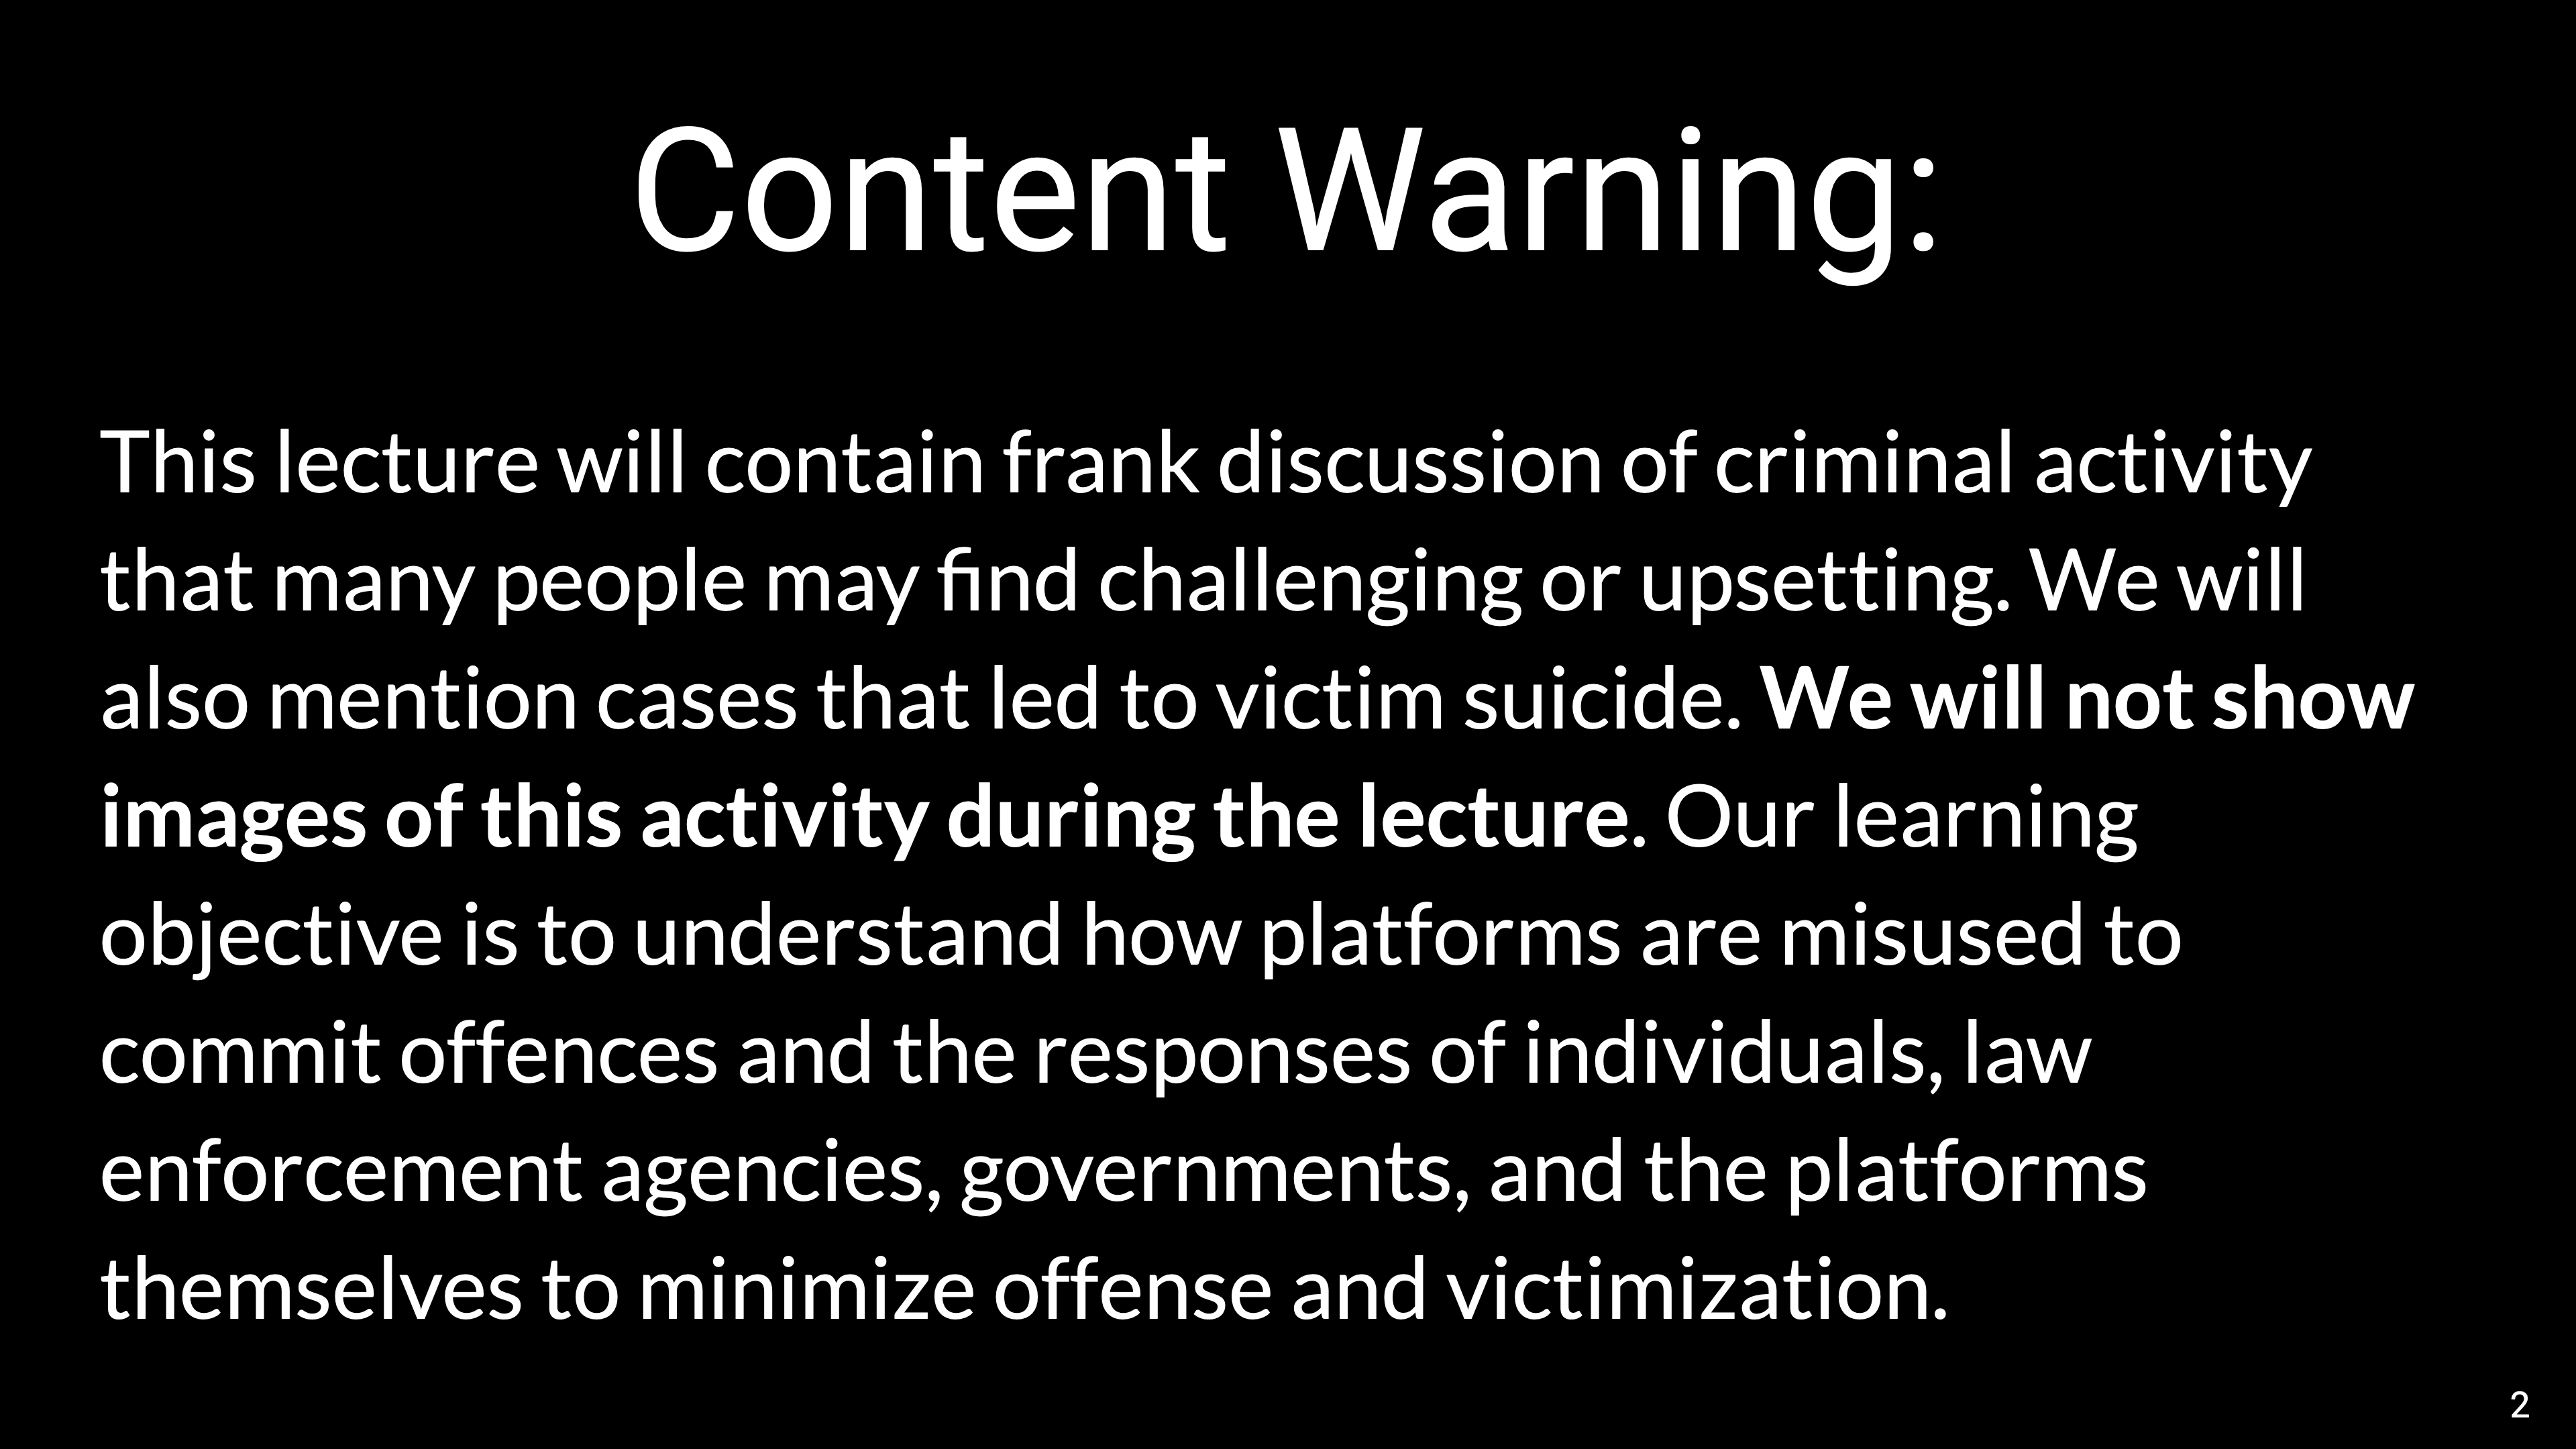
\includegraphics[width=\paperwidth]{content-warning}}
\end{frame}

\section{What Will We Discuss Today?}

\begin{frame}{What Will We Discuss Today?}
    \large
    \begin{itemize}
        \item How technology is misused by those seeking to exploit children
        \item How technology is deployed for good by those seeking to protect children
        \item Impacts of CSAM on victims
        \item NCMEC’s role in interfacing with tech companies, civil society, and law enforcement
        \item Modern responses to known CSAM
        \item Next week: grooming, sextortion and trafficking
    \end{itemize}
\end{frame}

\section{CSE and CSAM}

\begin{frame}{CSE and CSAM}
    \Large
    \underline{CSE}: \textit{\underline{C}hild \underline{S}exual \underline{E}xploitation}\\~\\
    \underline{CSAM}: \textit{\underline{C}hild \underline{S}exual \underline{A}buse \underline{M}aterial}
\end{frame}

\begin{frame}{How Does CSE Manifest Online?}
    \centering
    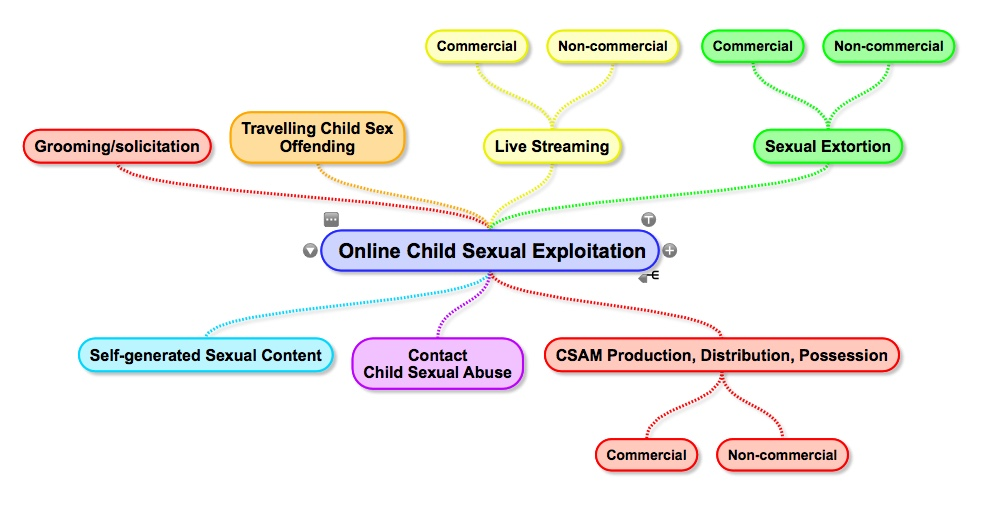
\includegraphics[width=\textwidth]{ocse}
    [Baines (2018)]
\end{frame}

\begin{frame}{How Does CSE Manifest Online?}
    \centering
    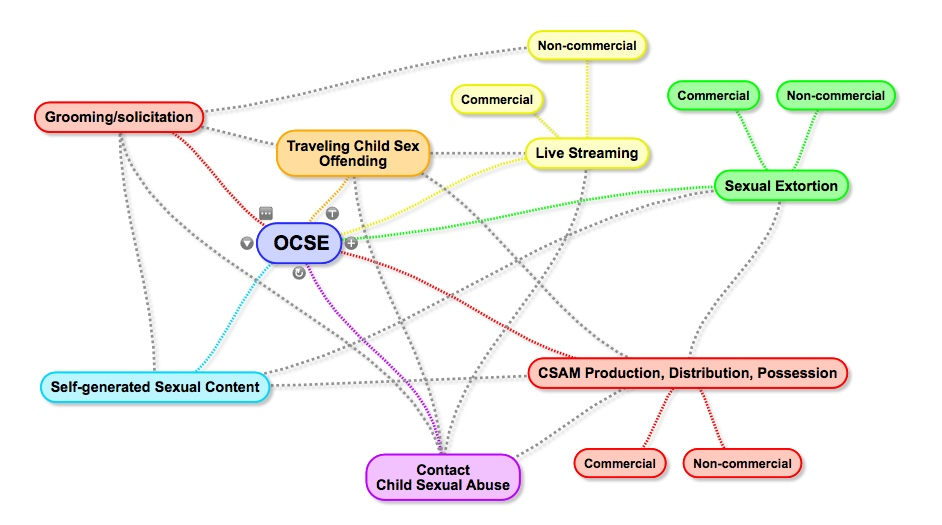
\includegraphics[width=0.95\textwidth]{ocse-2}
    [Baines (2018)]
\end{frame}

\begin{frame}{Where/How Are Offenses Committed?}
    \begin{columns}
        \column{0.5\textwidth}
            The short answer is: \textbf{everywhere.}\\~\\
            CSAM production:
            \begin{itemize}
                \item Abuse recorded offline, then distributed online
                \item Solicited/coerced online from children
            \end{itemize}
            CSAM distribution:
            \begin{itemize}
                \item Social platforms (“severe memes”)
                \item P2P filesharing - volume offending
                \item Dark Net and hidden services
                \item Commercial vs. non-commercial
                \item “Live streamed” abuse
            \end{itemize}
        \column{0.5\textwidth}
            
\includegraphics[width=0.9\textwidth]{everywhere}
    \end{columns}
\end{frame}

\begin{frame}{A Brief History: Five Overlapping Eras (Chad Steele)}
    Technology trends toward increased anonymity, storage, space and scale
    \begin{columns}[T]
        \column{0.2\textwidth}
            \textbf{1. The Networking Era} (1987-1996)
        \column{0.2\textwidth}
            \textbf{2. The Internet Goes Mainstream} (1996-2004)
        \column{0.2\textwidth}
             \textbf{3. Peer-to-Peer Software} (2004-2008)
        \column{0.2\textwidth}
             \textbf{4. Dark Web Technologies} (2008-2014)
        \column{0.2\textwidth}
             \textbf{5. Mobile Consumption} (2014-Present Day)
    \end{columns}
    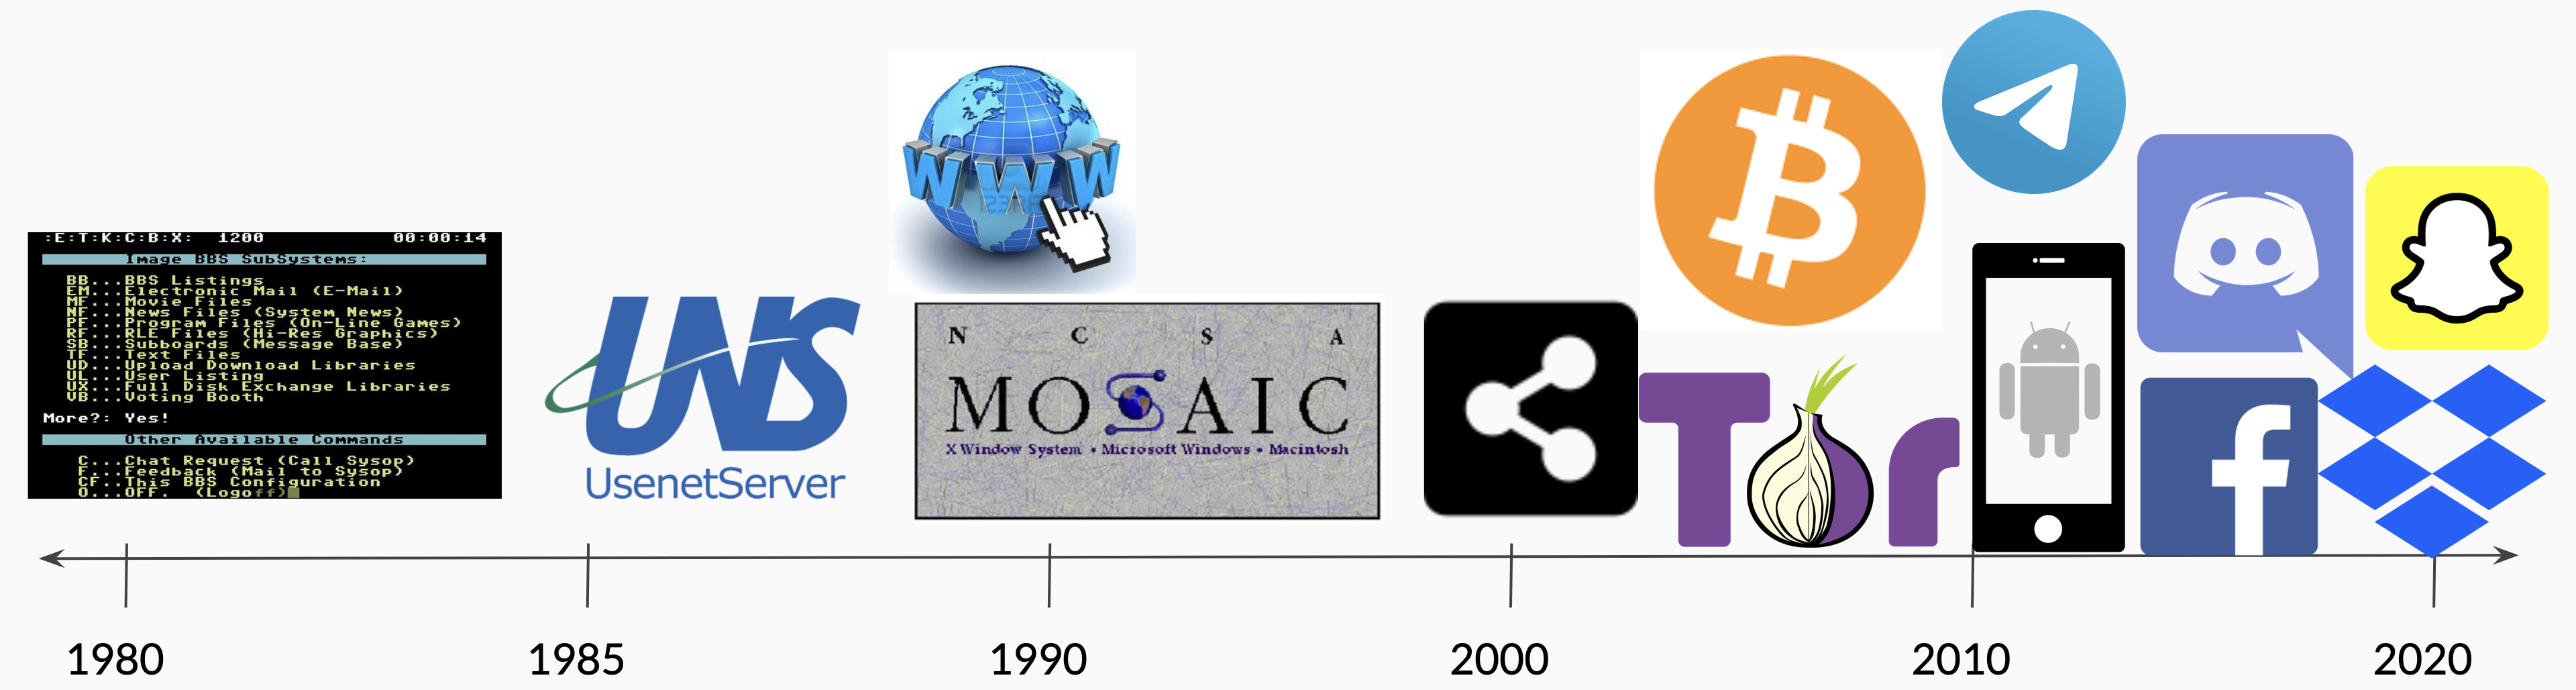
\includegraphics[width=\textwidth]{timeline}
\end{frame}

\begin{frame}{}
    \centering
    \Large{What makes CSE/CSAM different from other forms of abuse?}\\~\\
    \LARGE{\textbf{Everyone agrees it’s bad}}
\end{frame}

\begin{frame}{US CSAM Statutes}
    \begin{itemize}
        \item CSAM Statutes: 
        \begin{itemize}
            \item 18 U.S.C. 2252/2258A/2258B
            \item “Child porn statutes” (called CSAM by practitioners). 
        \end{itemize}
        \item Beyond \textbf{requirement to remove}, have a \textbf{reporting obligation}
    \end{itemize}
\end{frame}

\begin{frame}{Legal Definitions of CSAM: 18 USC §2256}
    For the purposes of this chapter, the term—
    \begin{enumerate}
        \item[(1)] “\underline{\href{https://www.law.cornell.edu/definitions/uscode.php?width=840&height=800&iframe=true&def_id=18-USC-103901109-1416780791&term_occur=999&term_src=title:18:part:I:chapter:110:section:2256}{minor}}” means any person under the age of eighteen years;
        \item[(2)(A)] Except as provided in subparagraph (B), “\underline{\href{https://www.law.cornell.edu/definitions/uscode.php?width=840&height=800&iframe=true&def_id=18-USC-821371409-1416780790&term_occur=999&term_src=}{sexually explicit conduct}}” means actual or simulated—
        \begin{enumerate}
            \item[(i)] sexual intercourse, including genital-genital, oral-genital, anal-genital, or oral-anal, whether between persons of the same or opposite \underline{\href{https://www.law.cornell.edu/definitions/uscode.php?width=840&height=800&iframe=true&def_id=18-USC-113766-970642657&term_occur=999&term_src=}{sex}};
            \item[(ii)]bestiality;
            \item[(iii)]masturbation;
            \item[(iv)]sadistic or masochistic abuse; or
            \item[(v)]lascivious exhibition of the anus, genitals, or pubic area of any person;
        \end{enumerate}
    \end{enumerate}
\end{frame}

\begin{frame}{Definitions - Lascivious}
    \small
    How do courts determine if a photo is lascivious exhibition?\\
    The “Dorr factors” are considered by the jury and judge:\\
    \begin{enumerate}
        \item Whether the focal point of the visual depiction is on the child's genitalia or pubic area.
        \item Whether the setting of the visual depiction is sexually suggestive, i.e., in a place or pose generally associated with sexual activity.
        \item Whether the child is depicted in an unnatural pose, or in inappropriate attire, considering the age of the child.
        \item Whether the child is fully or partially clothed, or nude.
        \item Whether the visual depiction suggests sexual coyness or a willingness to engage in sexual activity.
        \item Whether the visual depiction is intended or designed to elicit a sexual response in the viewer.
    \end{enumerate}
    \vspace{0.02\textheight}
    Do not need all factors, different courts use this is different ways
\end{frame}

\begin{frame}{Duty to Report}
    \begin{enumerate}
        \item[(a)]Duty To Report.—
        \begin{enumerate}
            \item[(1)]In general.—
            \begin{enumerate}
                \item[(A)]Duty.—In order to reduce the proliferation of online child sexual exploitation and to prevent the online sexual exploitation of children, a \underline{\href{https://www.law.cornell.edu/definitions/uscode.php?width=840&height=800&iframe=true&def_id=18-USC-987494927-970461075&term_occur=999&term_src=title:18:part:I:chapter:110:section:2258A}{provider}}—
                \begin{enumerate}
                    \item[(i)]shall, as soon as reasonably possible after obtaining actual knowledge of any facts or circumstances described in paragraph (2)(A), take the actions described in subparagraph (B); and
                    \item[(ii)]may, after obtaining actual knowledge of any facts or circumstances described in paragraph (2)(B), take the actions described in subparagraph (B).
                \end{enumerate}
                \item[(B)]Actions described.—The actions described in this subparagraph are—
                \begin{enumerate}
                    \item[(i)]providing to the CyberTipline of \underline{\href{https://www.law.cornell.edu/definitions/uscode.php?width=840&height=800&iframe=true&def_id=18-USC-74106838-970461074&term_occur=999&term_src=title:18:part:I:chapter:110:section:2258A}{NCMEC}}, or any successor to the CyberTipline operated by \underline{\href{https://www.law.cornell.edu/definitions/uscode.php?width=840&height=800&iframe=true&def_id=18-USC-74106838-970461074&term_occur=999&term_src=title:18:part:I:chapter:110:section:2258A}{NCMEC}}, the mailing address, telephone number, facsimile number, electronic mailing address of, and individual point of contact for, such \underline{\href{https://www.law.cornell.edu/definitions/uscode.php?width=840&height=800&iframe=true&def_id=18-USC-987494927-970461075&term_occur=999&term_src=title:18:part:I:chapter:110:section:2258A}{provider}}; and
                    \item[(ii)]making a report of such facts or circumstances to the CyberTipline, or any successor to the CyberTipline operated by \underline{\href{https://www.law.cornell.edu/definitions/uscode.php?width=840&height=800&iframe=true&def_id=18-USC-74106838-970461074&term_occur=999&term_src=title:18:part:I:chapter:110:section:2258A}{NCMEC}}.
                \end{enumerate}
            \end{enumerate}
        \end{enumerate}
    \end{enumerate}
\end{frame}%TODO2 error: too deeply nested?

\begin{frame}{Dimensions on Which CSAM Laws Vary}
    \begin{itemize}
        \item \textbf{Is there a law?} In 2018, most recent year for which we have data, 16 countries lacked laws specifically about CSAM (Iran, Iraq, Kuwait, Lebanon, Libya, etc - some prohibit all pornography, eg Iran)
        \item \textbf{Is CSAM defined?} 51 countries had laws but did not define CSAM
        \item \textbf{Is tech-facilitated CSAM prohibited?} 25 countries had laws but did not specify prohibition of technology-facilitated CSAM
        \item \textbf{Is possession prohibited?} 38 countries had laws but did not prohibit possession of CSAM (eg Russia)
        \item \textbf{Is fictional CSAM prohibited?} Variation in whether laws prohibit fictional CSAM (legal in Japan, Denmark, elsewhere)
        \item \textbf{Is ISP reporting required?}
    \end{itemize}
\end{frame}

\begin{frame}{Dimensions on Which CSAM Laws Vary}
    \centering
    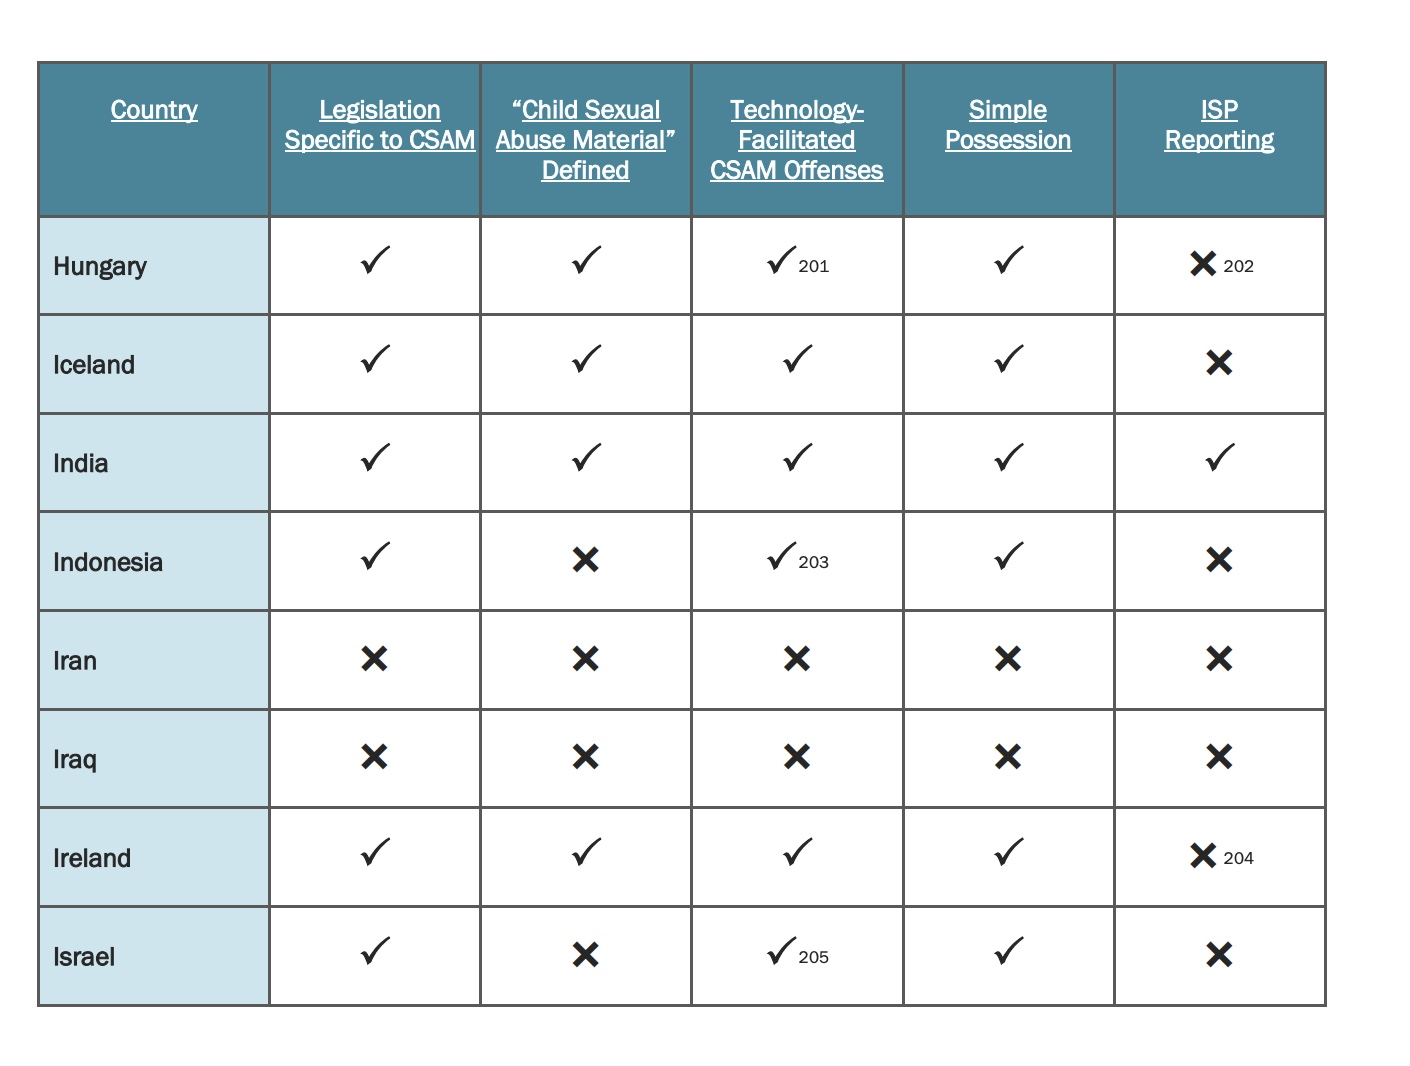
\includegraphics[width=0.8\textwidth]{varying-laws}
\end{frame}

\begin{frame}{What Does That Mean for Platform Policies?}
    \begin{itemize}
        \item Difficulty in determining lascivious means that many public platforms ban all photos of nude children
        \item Private services like iCloud Backup often do not have specific policies
        \item Public/private services like Google Photos might \_\_\_\_\_\_\_ all nudity but then apply a higher standard on sharing %TODO2 missing word?
        \item Many platforms only look for “worst” content
    \end{itemize}
\end{frame}

\begin{frame}{More than “Just Images”: Impacts on Victims}
    \begin{itemize}
        \item Every piece of CSAM can be linked to the exploitation of a child who was coerced or victimized into sharing a photo
        \item Saving and sharing such imagery extends the worst moment of victims’ lives 
        \item Viewing CSAM creates demand for more CSAM, which leads to more exploitation of children
    \end{itemize}
\end{frame}

\begin{frame}{Revictimization with Every Share}
    \textit{“I wonder if the men I pass in the grocery store have seen them. Because the most intimate parts of me are being viewed by thousands of strangers, and traded around, I feel out of control. They are trading my trauma around like treats at a party, but it is far from innocent. It feels like I am being raped by each and every one of them.”}\\~\\
    
    -\textit{Vicky (a pseudonym)}\\~\\
    \tiny
    \href{https://protectchildren.ca/en/programs-and-initiatives/project-arachnid/}{Project Arachnid}\\
    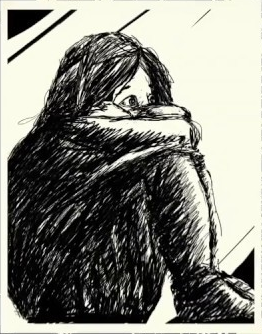
\includegraphics[width=0.175\textwidth]{sketch}
\end{frame}

\begin{frame}{Grading CSAM in Industry}
    \centering
    \begin{tabular}{|c|c|c|}%TODO2 table
        \hline
         & A & B\\
        \hline
        1 & Prepubescent minor, engaged in a sexual act & Pubescent minor, engaged in a sexual act\\
        \hline
        2 & Prepubescent minor, engaged in lascivious exhibition & Pubescent minor, engaged in lascivious exhibition\\
        \hline
    \end{tabular}
\end{frame}

\section{Reporting Obligation}

\begin{frame}{Absolutely Illegal}
    \Large
    \centering
    But what about Section 230 immunity???\\
    \textbf{\textit{Breaking federal criminal law is NOT immunized by Section 230.}}\\
    \textbf{\textit{CSAM, terrorism, trafficking, etc.}}
\end{frame}

\begin{frame}{National Center for Missing and Exploited Children (NCMEC)}
    \centering
    \begin{figure}
        \centering
        
\includegraphics[width=0.5\textwidth]{ncmec}
    \end{figure}
    \begin{figure}
        \centering
        
\includegraphics[width=0.5\textwidth]{report-cse}
    \end{figure}
    \textit{National resource center and clearinghouse for CSAM, which is otherwise illegal to hold.}
\end{frame}

\begin{frame}{Modern Responses to Known CSAM}
    \centering
    \adjincludegraphics[trim=0 25 0 20, clip, width=\textwidth]{cybertipline-workflow}
\end{frame}

\begin{frame}{How Big Is the Problem?}
    \begin{columns}
        \column{0.6\textwidth}
            NCMEC CyberTipline Reports from 2014 - 2020\\
            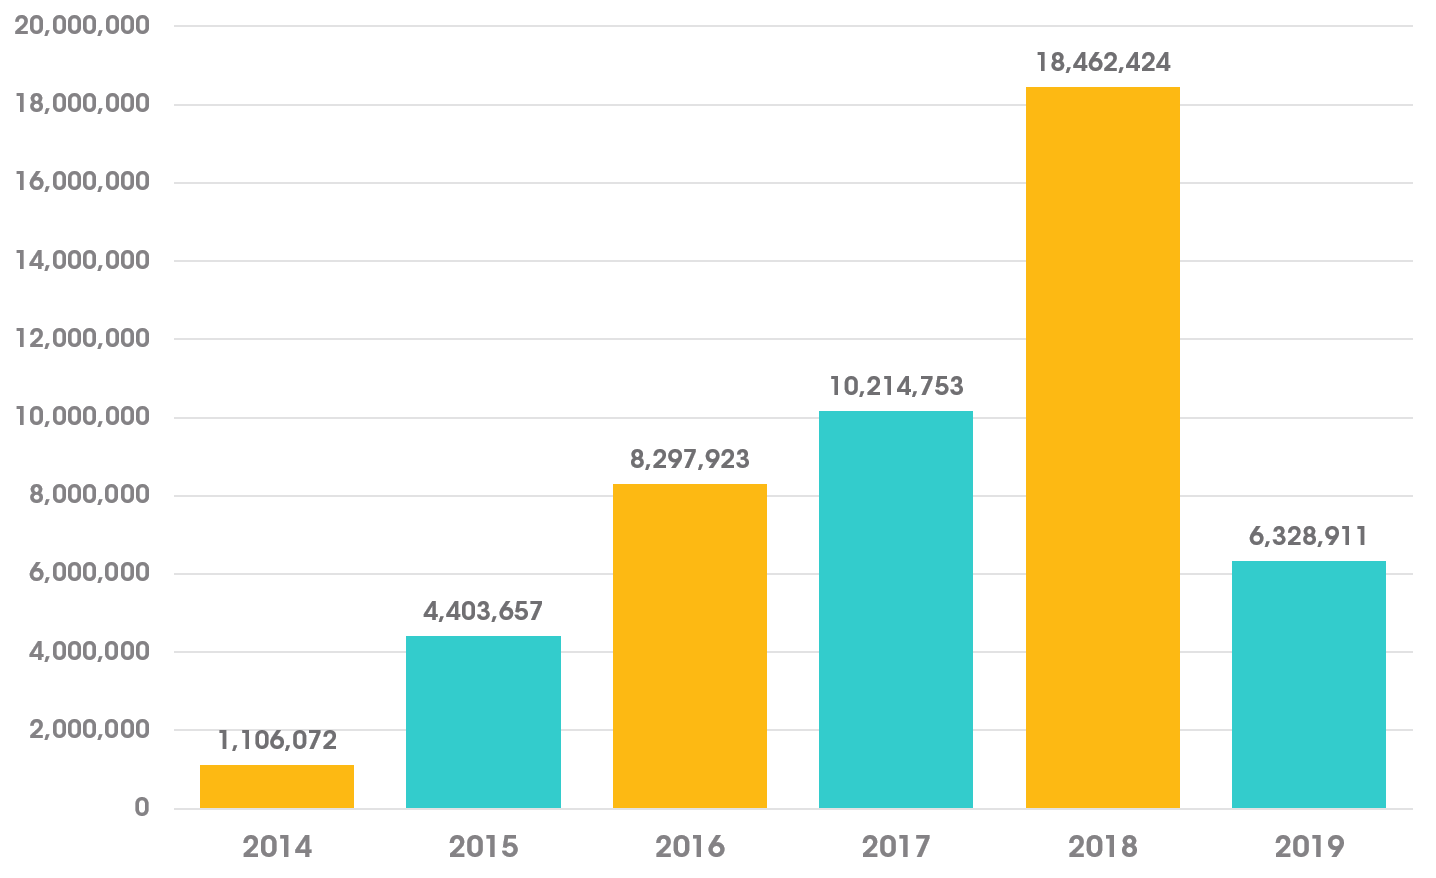
\includegraphics[width=\textwidth]{cybertipline-reports-2014-2018}
        \column{0.4\textwidth}
            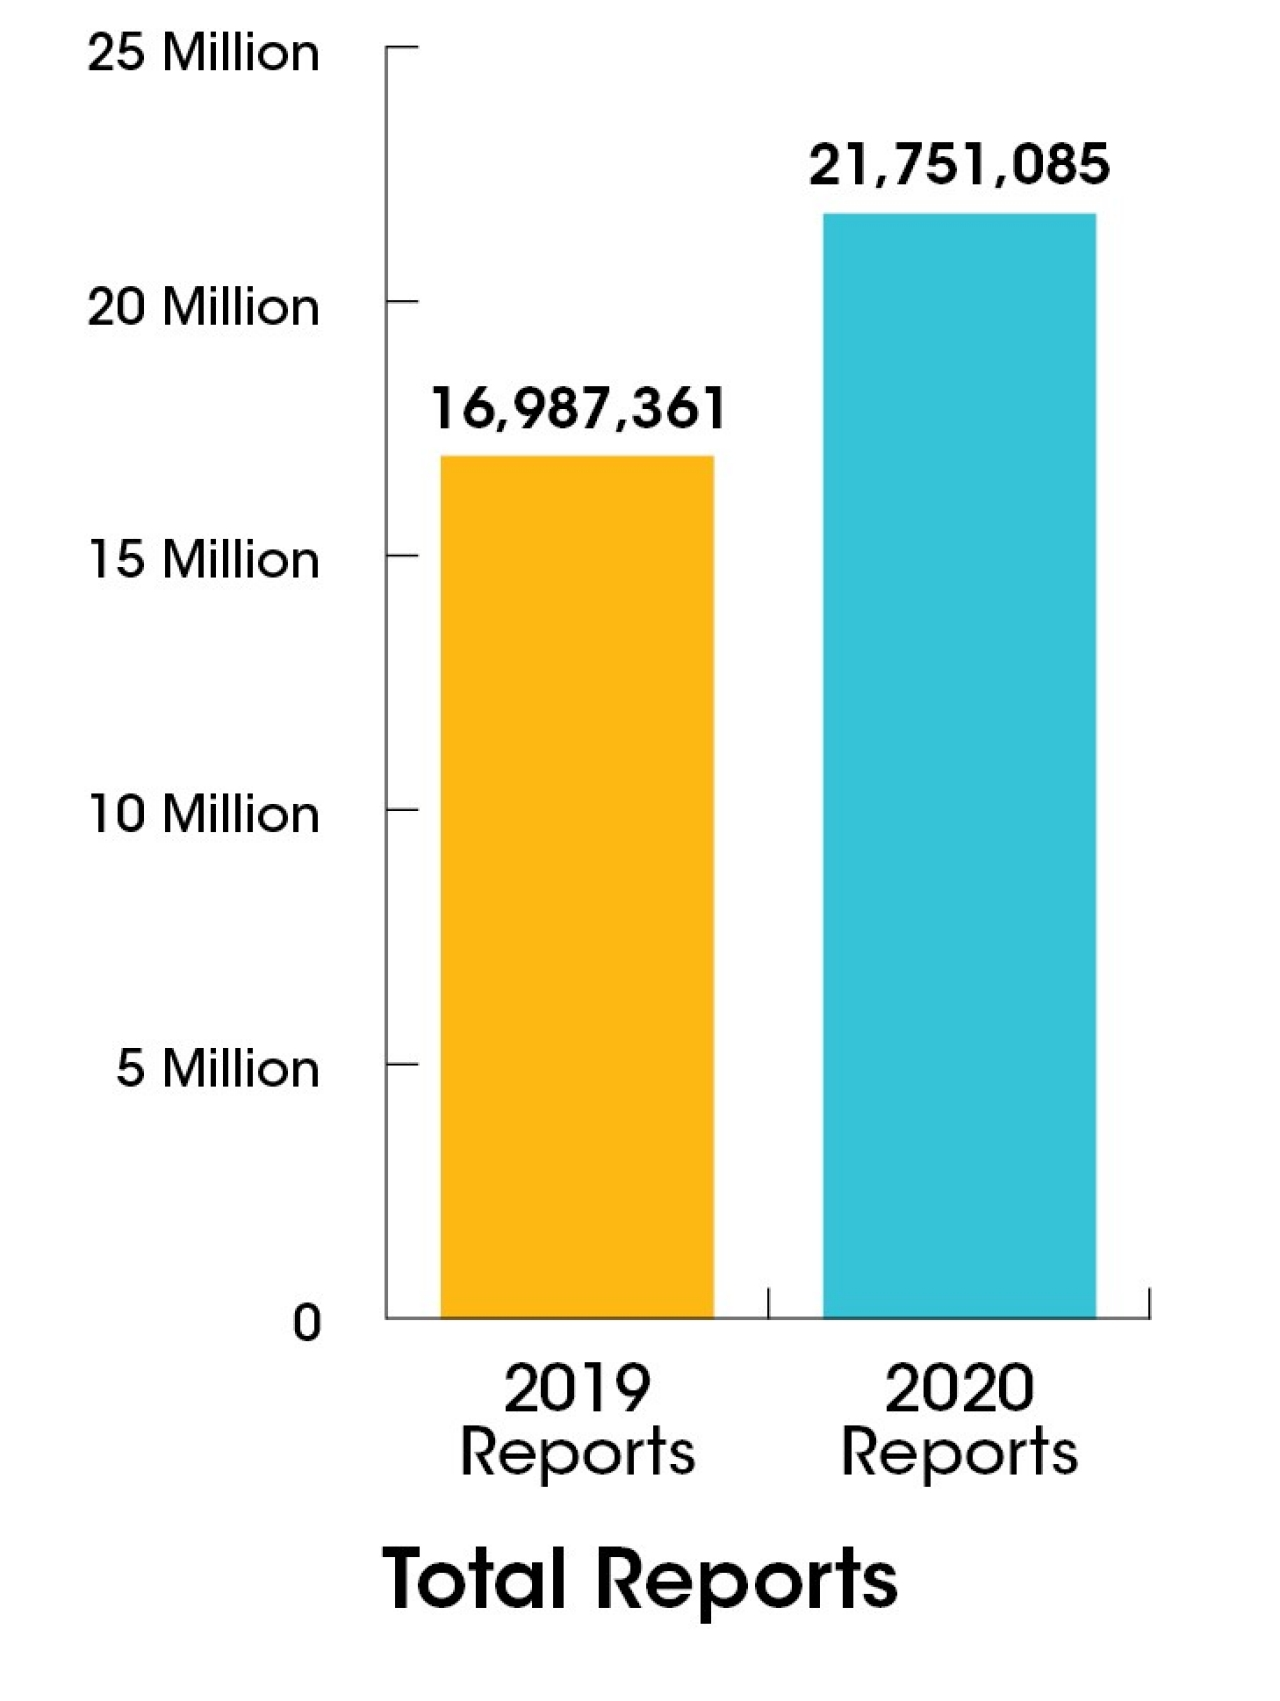
\includegraphics[width=\textwidth]{cybertipline-reports-2019-2020}
    \end{columns}
\end{frame}

\begin{frame}{Vast Majority Are the Trading of Known CSAM}
    %TODO2 title missing word? vast majority of what?
    \centering
    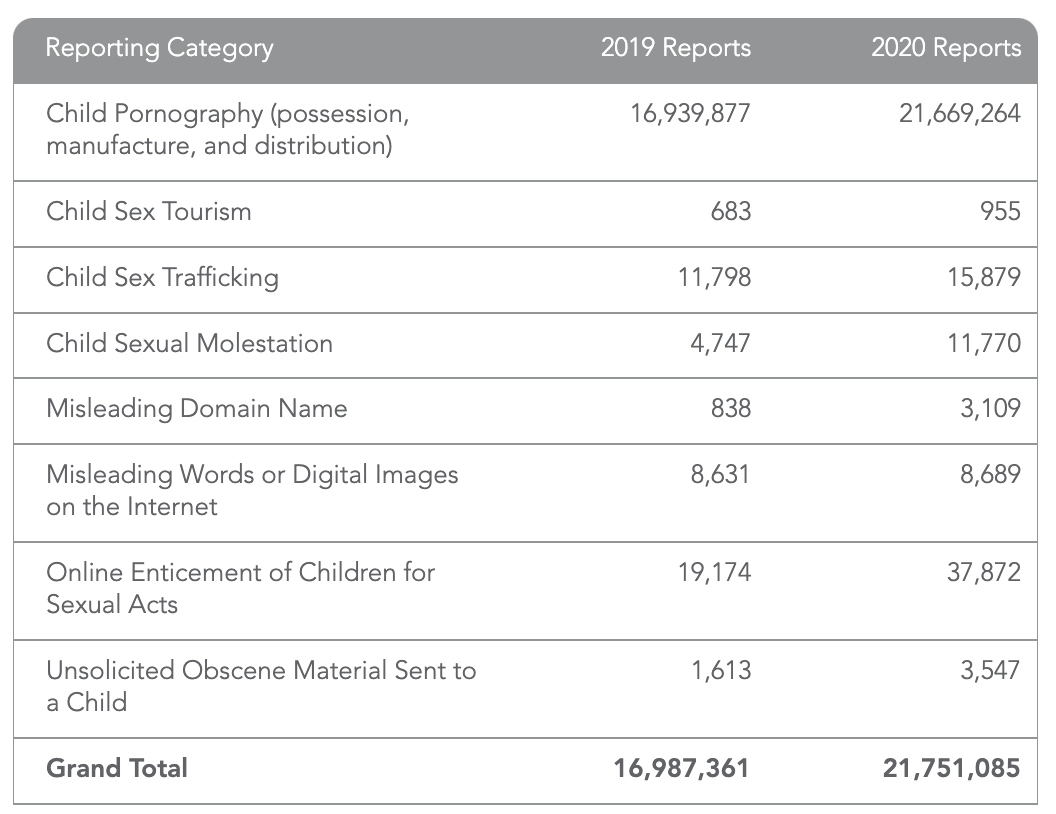
\includegraphics[width=0.6\textwidth]{reporting-categories}
\end{frame}

\begin{frame}{Majority of Reports by ESPs Regarding International Cases}
    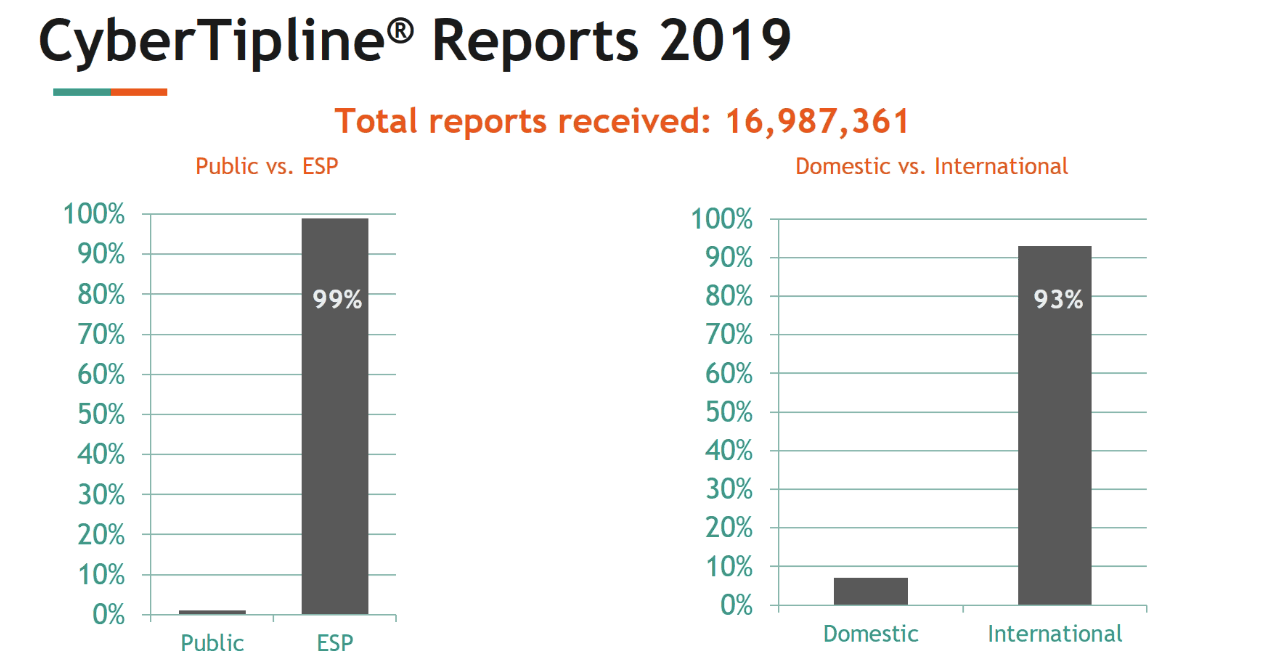
\includegraphics[width=\textwidth]{cybertipline-esp-reports-mostly-international}
\end{frame}

\begin{frame}{}
    \thispagestyle{empty}
    \AddToShipoutPictureBG*{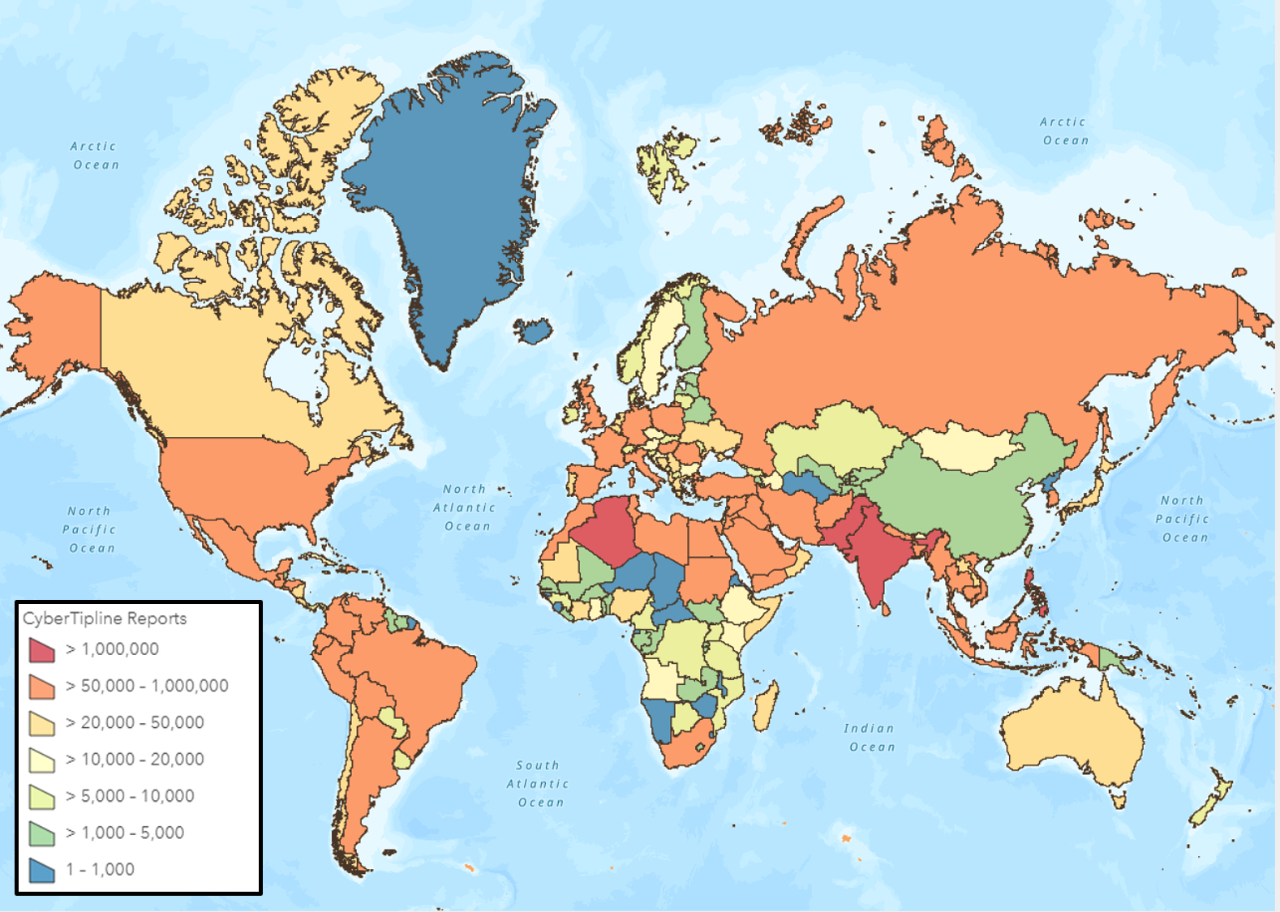
\includegraphics[width=\paperwidth]{cybertipline-reports-map}}
\end{frame}

\begin{frame}{Motivations for Uploading CSAM}
    \textbf{“Malicious” users}
    \begin{itemize}
        \small
        \item Preferential offenders (motivation: sexual interest in children)
        \item Commercial offenders (financial motive)
        \item Situational offenders (opportunistic)
    \end{itemize}
    \textbf{“Nonmalicious” users}
    \begin{itemize}
        \small
        \item Unintentional offenders (sharing image with statement of abhorrence; meme; vigilante)
        \item Minor nonexploitative users (eg sexting between teens)
        \item Situational “risky” offenders  (sharing adult pornography, that included an image of a child, maybe a 16 year old who might look like an adult)
    \end{itemize}
    \small
    “We evaluated 150 accounts that we reported to NCMEC for uploading CSAM in July and August of 2020 and January 2021, and we estimate that more than \textbf{75\% of these did not exhibit malicious intent} (i.e. did not intend to harm a child), but appeared to share for other reasons, such as outrage or poor humor.”
    \tiny
    \url{https://research.facebook.com/blog/2021/02/understanding-the-intentions-of-child-sexual-abuse-material-csam-sharers/}
\end{frame}

\begin{frame}{}
    \centering
    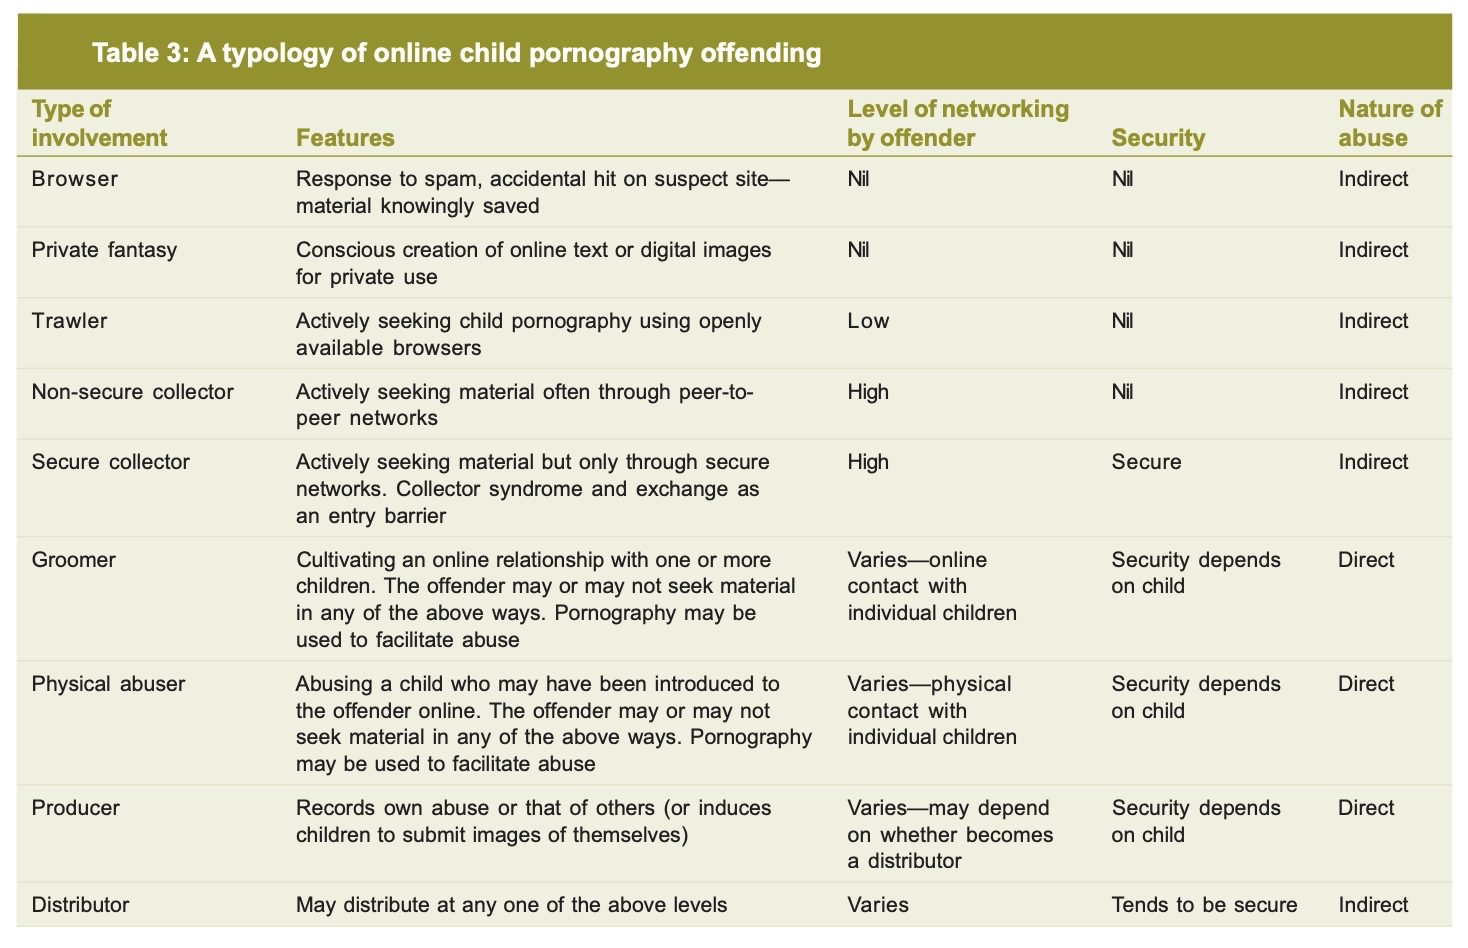
\includegraphics[width=\textwidth]{typology-of-ocse-offenders}
\end{frame}

\section{Responses and Mitigations}

\begin{frame}{Policy Responses}
    \large
    \begin{enumerate}
        \item Reach out to NCMEC early
        \item Create detailed policies for relevant type of CSAM/CSE
        \item Enlist lawyers and policy teams who understand this area
        \item Invest in coordinating bodies
        \item Publish transparency reports on child harm
        \item Create resiliency programs for employees working on these issues
    \end{enumerate}
\end{frame}

\begin{frame}{A Global Phenomenon That Requires a Global Response}
    \begin{itemize}
        \item Content and illegal activity does not respect national borders
        \item Governments, Companies, NGOs, helplines, tiplines all need to work together
    \end{itemize}
    
\includegraphics[width=\textwidth]{organizations}
\end{frame}

\begin{frame}{Responding to CSE}
    \centering
    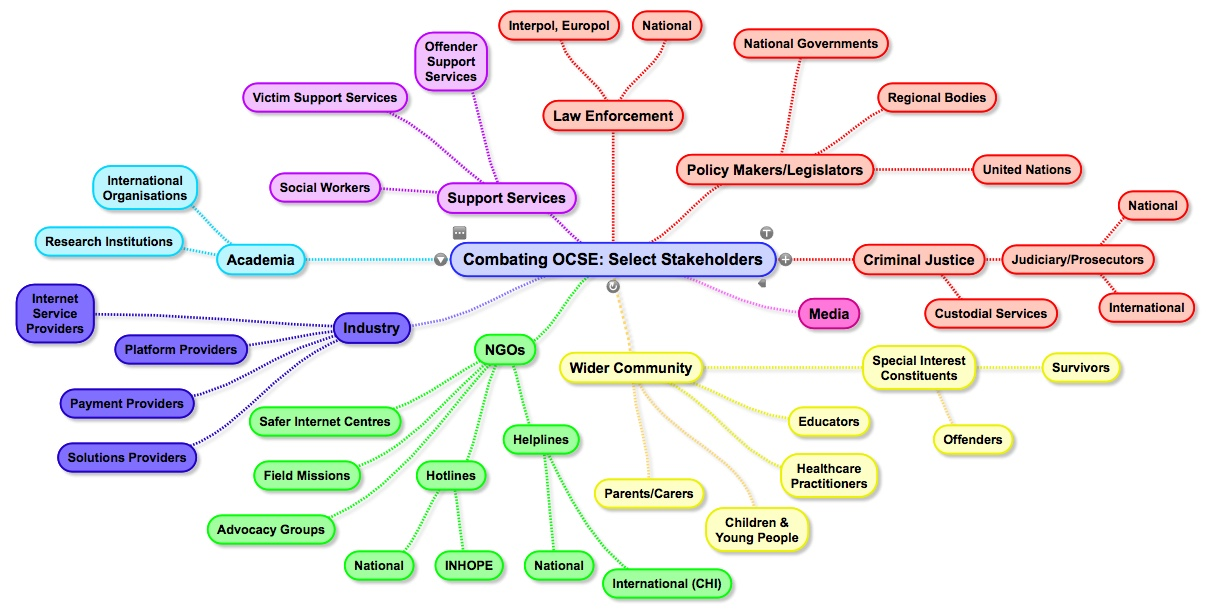
\includegraphics[width=\textwidth]{responding-to-ocse}
    [Baines (2018)]
\end{frame}

\begin{frame}{Product/Technical Responses}
    \large
    \begin{enumerate}
        \item Proactively detect and report known CSAM
        \item Provide reporting mechanisms for users and victims
        \item Flag potential grooming behaviors using known indicators
        \item Enforce identity indicators around age
        \item Restrict discovery of children by unfamiliar adults
    \end{enumerate}
\end{frame}

\begin{frame}{PhotoDNA}
    \centering
    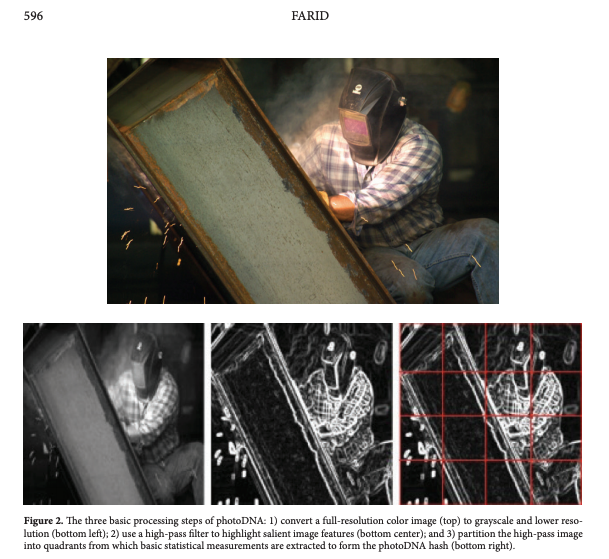
\includegraphics[width=0.6\textwidth]{photodna}
\end{frame}

\begin{frame}{Perceptual Hashes vs. Manipulation}
    \begin{columns}
        \column{0.5\textwidth}
            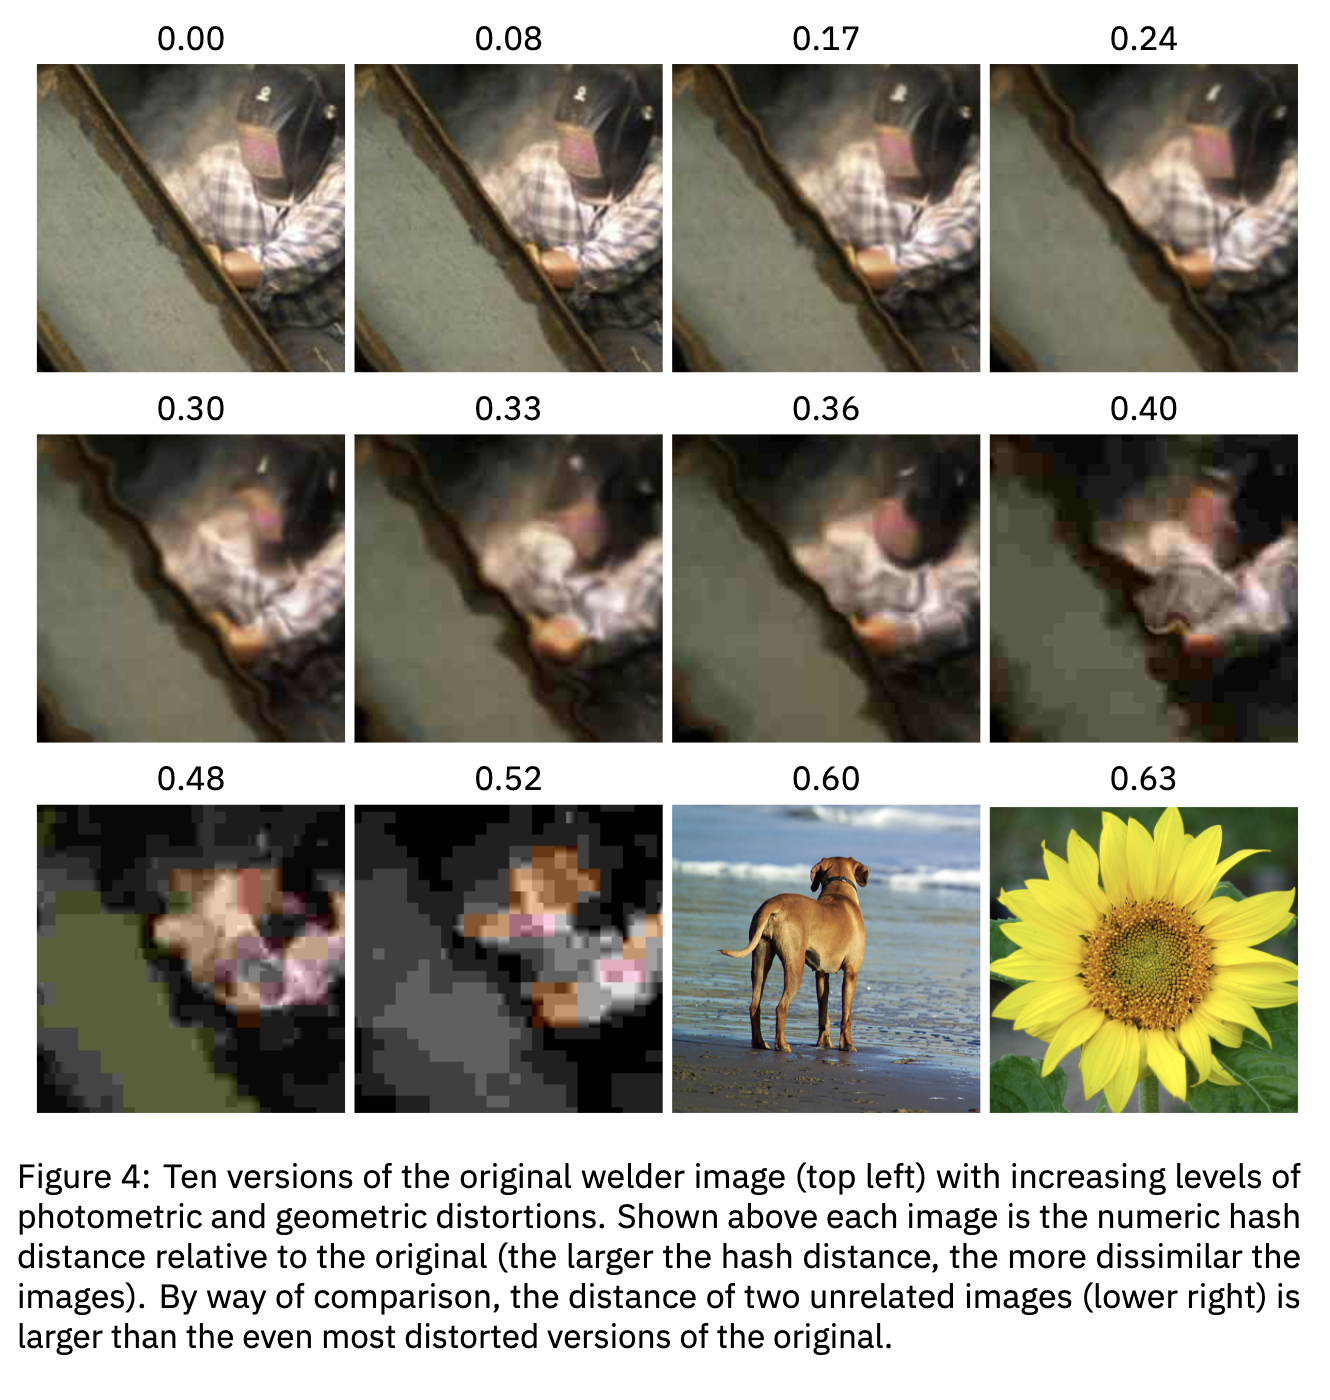
\includegraphics[width=0.9\textwidth]{perceptual-hashes-vs-manipulation-1}
            \tiny
            \url{https://tsjournal.org/index.php/jots/article/view/24/14}
        \column{0.5\textwidth}
            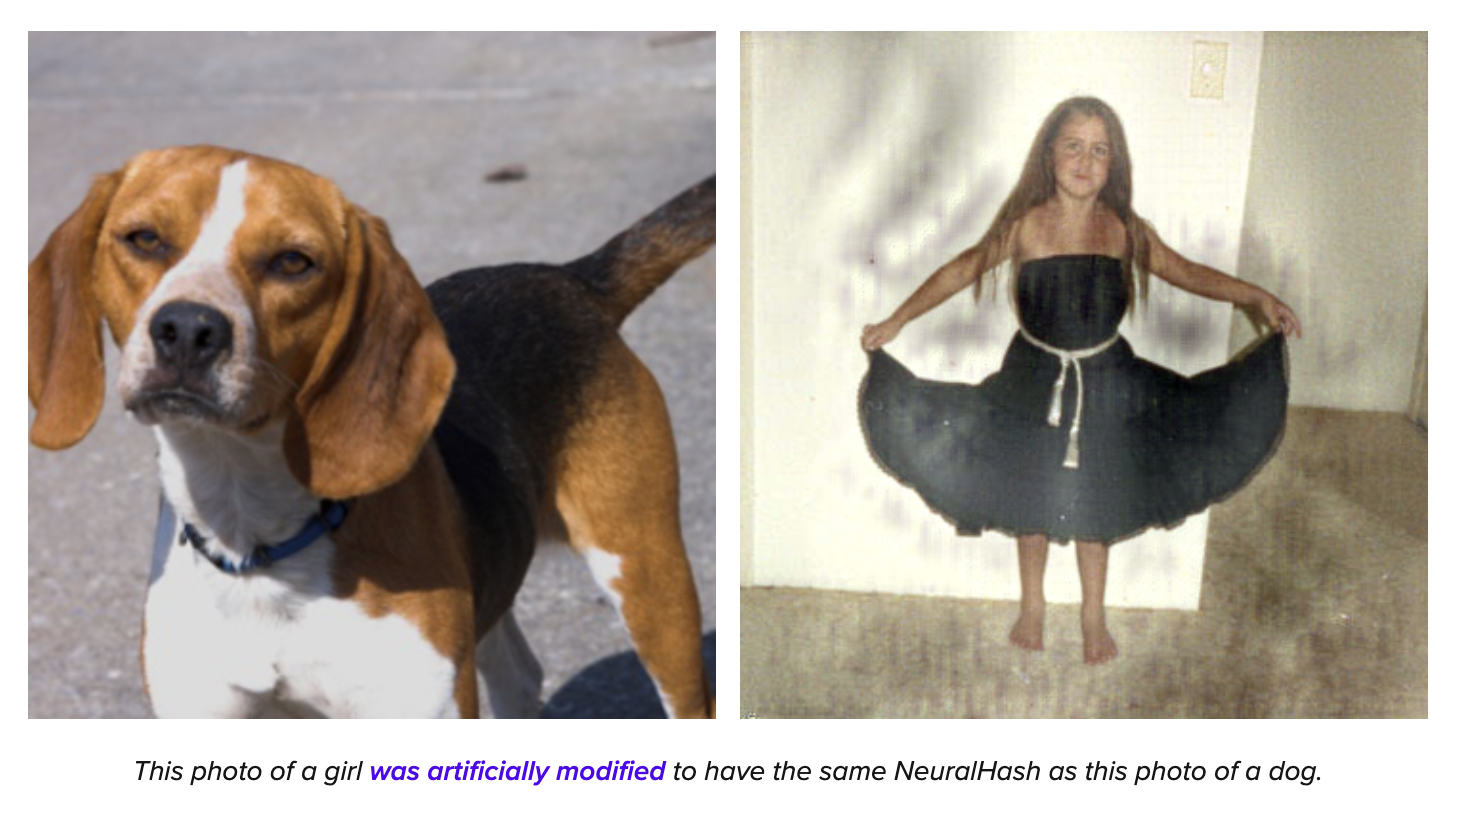
\includegraphics[width=\textwidth]{perceptual-hashes-vs-manipulation-2}
            \tiny
            \url{https://blog.roboflow.com/neuralhash-collision/}
    \end{columns}
\end{frame}

\begin{frame}{Automated Classification vs. Human Review}
    Autmated Classification:
    \begin{itemize}
        \item Tools like PhotoDNA are great at identifying known images if they’re fed the correct hashes.
        \item But what about new CSAM generated by children who have been groomed or coerced online?
        \item Is there more we can do to intervene before material is shared, i.e. in the “chat” phase?
    \end{itemize}
    Human review, meanwhile is:
    \begin{itemize}
        \item Fallible and time consuming
        \item Liable to be challenged by cultural differences (so is technology)
        \item Emotionally tough, requiring companies to think about their reviewers’ resilience and well-being.
    \end{itemize}
\end{frame}

\begin{frame}{Privacy and Safety}
    Why are there trade offs in designing for user privacy and designing for user safety?
\end{frame}

\begin{frame}{The Apple Controversy}
    \begin{columns}
        \column{0.6\textwidth}
            \begin{itemize}
                \item Apple announces plan to: 
                \begin{itemize}
                    \item Alert parents when child sends or receives nude photo on iMessage
                    \item Blur nude photos children receive
                    \item Scan iCloud Photos (on device) for known CSAM
                    \begin{itemize}
                        \item Report to NCMEC if threshold is reached
                    \end{itemize}
                \end{itemize}
                \item Criticisms:
                \begin{itemize}
                    \item Known CSAM dataset could be expanded to include…political dissent images
                    \item Apple says it will let outsiders audit the image dataset, but they don’t have a reputation for doing this
                    \item Parental alert could out a child
                \end{itemize}
            \end{itemize}
        \column{0.3\textwidth}
            \centering
            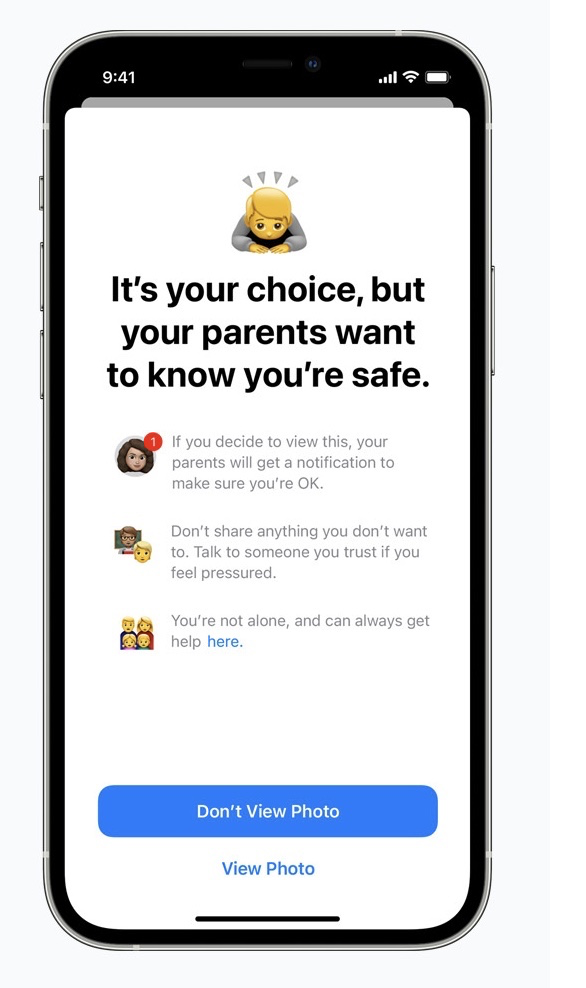
\includegraphics[width=\textwidth]{apple-controversy-1}
            (original proposal)
    \end{columns}
\end{frame}

\begin{frame}{What Apple Does Now}
    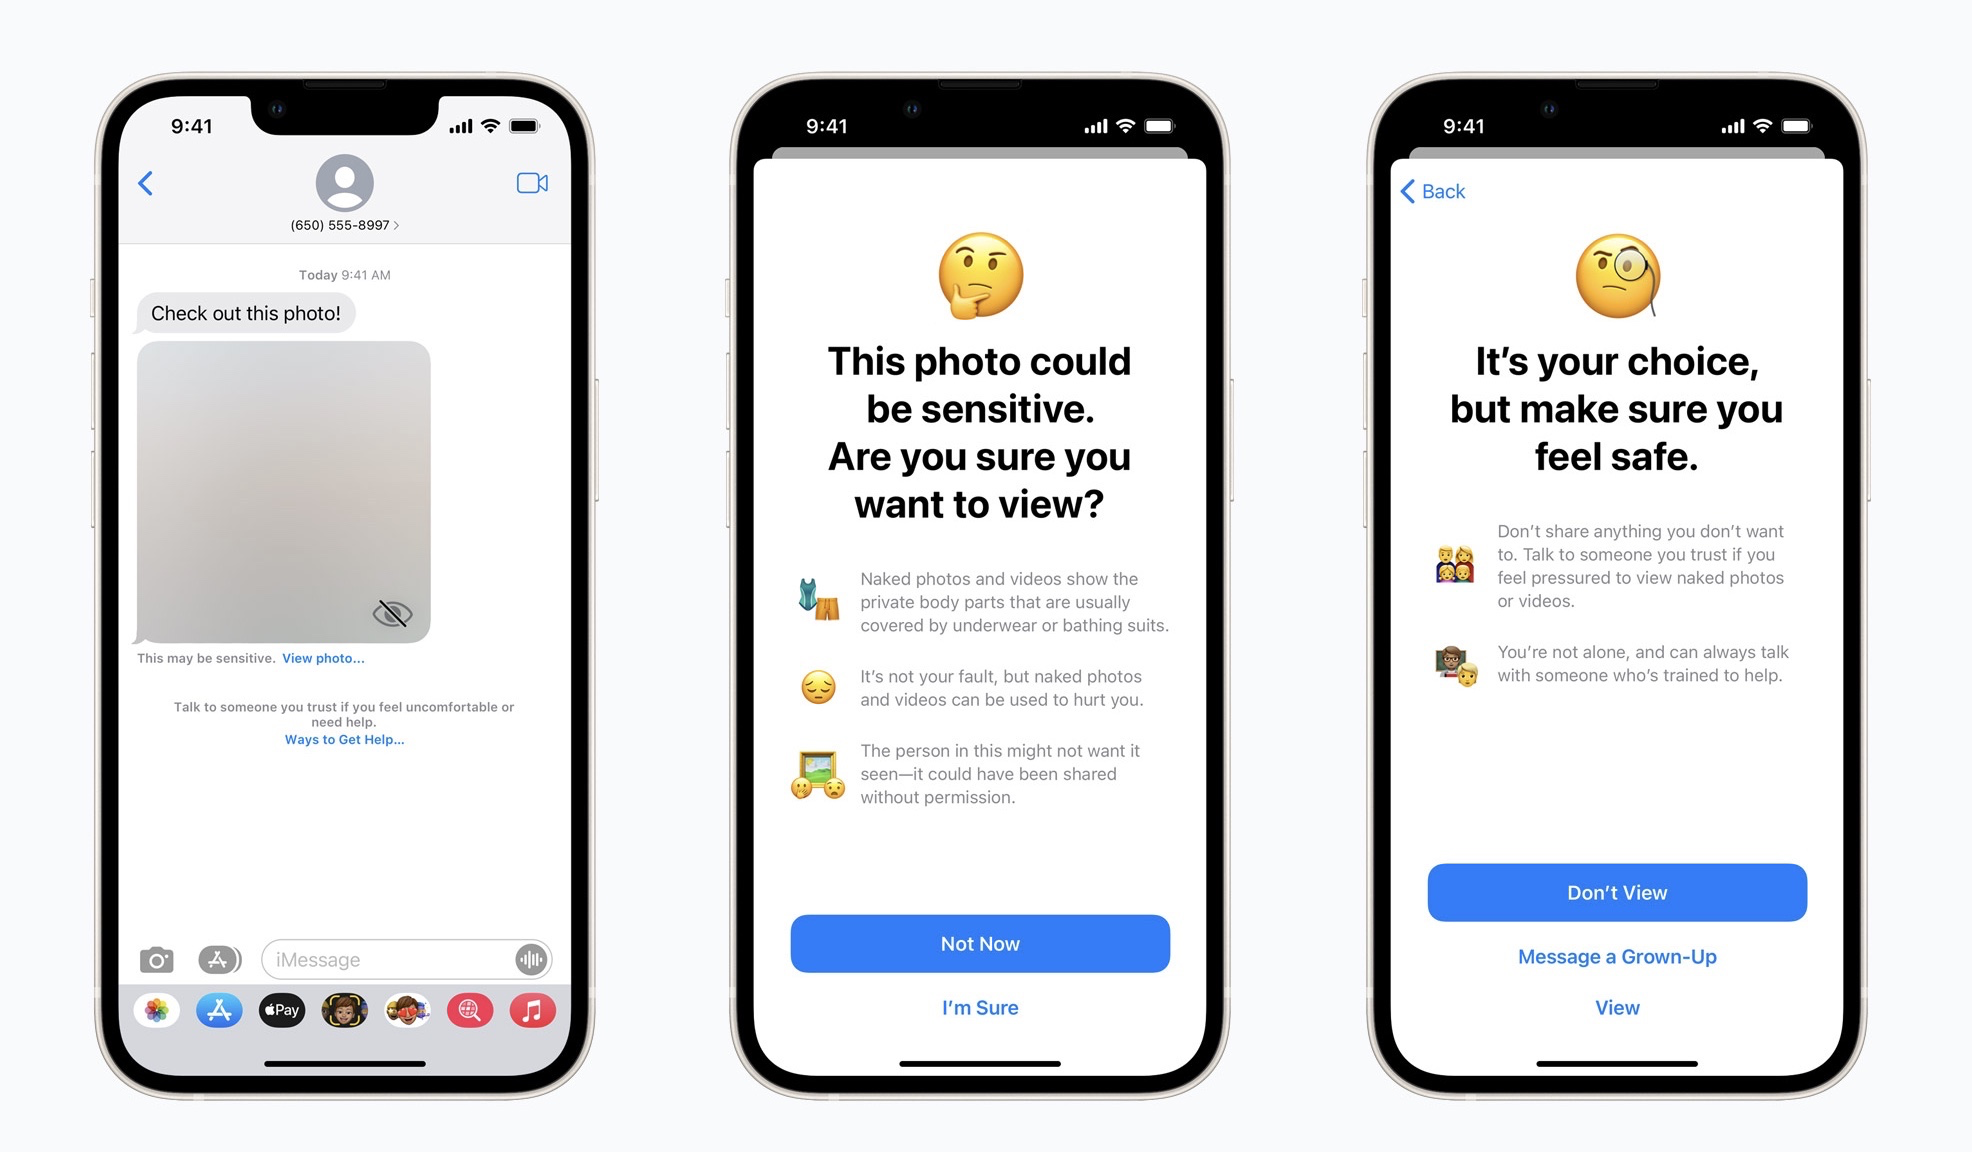
\includegraphics[width=0.99\textwidth]{apple-controversy-2}
\end{frame}

\begin{frame}{What WhatsApp Does}
    \begin{itemize}
        \item Scan profile and group photos
        \item Examine reported content
        \item Machine learning classifiers scan unencrypted text (e.g. group description)
        \item WhatsApp says they ban 300,000 accounts for CSAM activity per month
        \item Receive tips from law enforcement when WhatsApp links found in dark web forums
    \end{itemize}
\end{frame}

\begin{frame}{Privacy and Safety Sometimes Go Together}
    “Meta must also limit recommendation engines and discoverability. “People You May Know” has for years been understood as problematic within Facebook for its propensity to make inappropriate suggestions: recommending a therapist’s clients to each other, or potential targets to a possible abuser.”\\~\\
    “One way to prevent such features from leading to unwanted and unsafe social connections would be to make it so that users with no social connection or those surfaced via search or People You May Know can start chats without end-to-end encryption, and then have the option to mutually opt in.”\\~\\
    -David Thiel
\end{frame}

\begin{frame}{CSE as a Public Health Issue}
    An important distinction: not all sex offenders who target children are pedophiles, and not all pedophiles commit sexual offenses.
    \begin{itemize}
        \item Wurtele et al. (2014): Among men, 6\% indicated some likelihood of having sex with a child if they were guaranteed they would not be caught or punished, as did 2\% of women. Nine percent of males and 3\% of females indicated some likelihood of viewing CSAM on the Internet. Overall, nearly 10\% of males and 4\% of females reported some likelihood of having sex with children or viewing CSAM.
        \item Self-report perpetration surveys conducted in Australia, Canada, Sweden, the UK and the US show that between 4\% (Seto et al., 2014) and 12\% of men, and 3\% of women in the general population engage with CSAM (Seigfried-Spellar, 2014). [Reported in Wager et al. 2018]
    \end{itemize}
\end{frame}

\end{document}